% Template - https://sanskrit.uohyd.ac.in/18WSC/Style_files/CS_and_DH.tex
\providecommand{\tightlist}{%
  \setlength{\itemsep}{0pt}\setlength{\parskip}{0pt}}

\documentclass[11pt]{article}
\usepackage{scl}
\usepackage{times}
\usepackage{url}
\usepackage{latexsym}
\usepackage{lineno}

\usepackage{fontspec, xunicode, xltxtra}
\newfontfamily\skt[Script=Devanagari]{Sanskrit 2003}
\setmonofont{Sanskrit 2003}


\title{A universal subhāṣita database, and deduplicating sanskrit texts}

\author{Vishvas Vasuki \\
  Dyugaṅgā, Beṅgaḷūru - 92 \\
  {\tt vishvas.vasuki+ACAD@gmail}
\\}

\date{}

\begin{document}
\maketitle
%\linenumbers
\begin{abstract}
Subhāṣita-s are popular and beautiful Sanskrit quotations. In this paper, we propose a universal open-source subhāṣita database. As a part of it, we present an algorithm for deduplicating sanskrit texts, as well as one for identifying non-duplicate vairants of a given quote.
\end{abstract}

\section{Motivation}
Subhāṣitas are popular and beautiful Sanskrit quotations - they're usually verses. One of the greatest (and useful) pleasures I've had in tough times is retreat for a while into the world of beautiful Subhāṣitas- so as to burst forth with renewed wisdom and energy. 

Since ages, they have been lovingly compiled [E.g. \cite{subhashita-1952}, \cite{mss-1974}] and memorized. I especially like online collections curated by some friends and myself since a book is not always available, and I want to collect + easily access choice ones for future enjoyment. But it is tedious (atleast for me) to sit in front of a computer to do the following:

\begin{itemize}
\tightlist
\item
  read them,
\item
  or scour the internet for new ones
\item
  or collect favorites in a spreadsheet
\item
  or just annotate them with comments.
\end{itemize}

So, it is desirable to make the above as simple and easy as possible, and to share our collective labor so that we can benefit more easily from each others' work.

\section{A universal database}

We've set out to build a database of Subhāṣitas - which is:

\begin{itemize}
\tightlist
\item
  \textbf{Universal}

  \begin{itemize}
  \tightlist
  \item
    Its goal is to contain within it every worthy Subhāṣita ever
    composed.
  \item
    In fact, the ultimate ambition encompasses all languages, verse
    and prose forms.
  \end{itemize}

\item
  \textbf{Freely and easily available}.

  \begin{itemize}
  \tightlist
  \item
     Anyone should be able to access it.
  \item
     Anyone should be able to copy and export it to other formats, thereby making it robust to network delays and geopolitical blockage\footnote{For example, unprecedented restrictions - and even "cancellations" - were imposed on Russian users, sportsmen and artists (both living and long dead) by several Western institutions and internet services in the wake of Western sanctions against Russia around March 2022.}. 
  \item
     Anyone should be able to present it in any way users will find convenient.
  \item
     Anyone should be able to suggest corrections and annotations. 
  \item
     Maintenance and serving the database should be possible with very low (Ideally 0) budget. 
  \end{itemize}
\item
  \textbf{Growing constantly in number}, thanks to contemporary compositions.
\item
  \textbf{Growing constantly in annotations}, where annotations include ratings, description, translations, metre, flaws, sources \ldots.
\end{itemize}

\section{Implementation}
\subsection{The database}
We have implemented the proposed database as a simple collection of markdown files with TOML metadata. This database is located at \url{https://github.com/subhAShita/db_toml_md__sa__padya} . The database is hosted at the popular  github.com. The database itself is version controlled - so that one can view a history of changes made pertaining to any quote. Anyone can suggest additions or other corrections to the database via the well-known mechanism of Github pull requests. Such requests can then be reviewed and accepted by the database maintainers.

As of 19 March 2022, the database consists of about 19k verses - mostly from secondary sources such as \cite{subhashita-1952} and \cite{mss-1974}. Metrical distribution is shown below.

\begin{figure}[h]
\caption{Mechanically deduced metrical distribution}
\centering
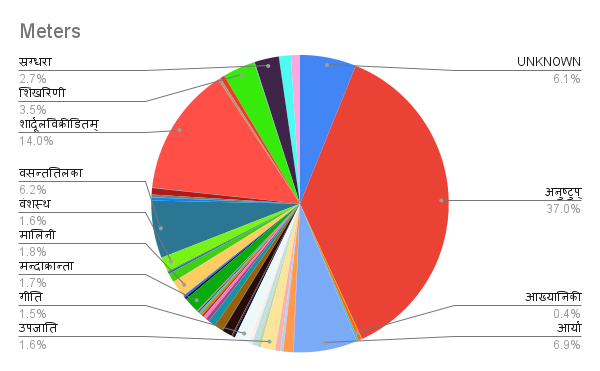
\includegraphics[width=1.0\textwidth]{Meters}
\end{figure}

\subsection{Entry format}
In describing the essentials of the file format we've settled upon, it is best to start with examples. A typical entry, showing two variants of the same verse, is shown below:

\begin{verbatim}
File path: main/A/y/u/S/h/AyuShaHxamaekopisarv_1.md
+++
topics = [ "कालः", "आयुः",]
ratings = [ "vvasuki:5",]
secondary_sources = [ "MSS_5160",]
meters = [ "अनुष्टुप् (श्लोक)",]
jsonClass = "Subhaashita"
title = "आयुषः क्षण"

+++

<details open><summary>Text</summary>

आयुषः क्षण एकोऽपि सर्वरत्नैर्न लभ्यते।  
नीयते यद् वृथा सोऽपि प्रमादः सुमहानयम्॥
__________________
आयुषः क्षण एकोऽपि सर्वरत्नैर्न लभ्यते।  
नीयते स वृथा येन प्रमादः सुमहानहो ॥
</details>

\end{verbatim}

Another example, from the gifted contemporary poet Shankar Rajaraman, recording a note from an unknown source - 

\begin{verbatim}
File path: main/g/a/j/A/m/gajAmamasy.md
+++
topics = [ "गणेशः",]
sources = [ "राजारामज-शङ्करः - मुक्तकम्",]
ratings = [ "vvasuki:5",]
meters = [ "अनुष्टुप् (श्लोक)",]
jsonClass = "Subhaashita"
title = "गजाननस्य जीयासुः"

+++

<details open><summary>Text</summary>

गजाननस्य जीयासुः कर्णतालझलज्झलाः ।  
श्रुत्यन्तवचनैर्यासामनुवादो विधीयते ॥
</details>



<details><summary>अज्ञात-विवरणम्</summary>

श्रुत्यन्तशब्दे श्लेषः।
</details>
\end{verbatim}

\section{Expected extensions}
We hope that this will motivate other such long-sought-after universal databases for sanskrit connoiseurs, like: one for metres.

The front-end clients built for this database could serve as a model for other kāvya readers. Similarly, one can build a collaboratively annotated and rated collection of verses/ sentences within the context of long sequential works (rather than free floating subhāṣitas).

% include your own bib file like this:
\bibliographystyle{acl}
\bibliography{scl}
\end{document}